\section{Merging of Datasets}

Following curation of individual datasets, these will need to be merged to homogenise variant calls across all data, and generate a square matrix of variant calls, where the union of variants across all samples is available for each population. In order to do this, a union set of calls will be generated for variants that have passed filtering in each dataset (Figure 1). Prior to merging 1) indels will be left aligned (e.g. bcftools norm), 2) SNPs and indels called in low coverage data by UnifiedGenotyper will be merged into single records with bcftools (bcftools norm -m +any) and 3) variants called from reads aligned to build 38 will be lifted over to build 37 (liftOver). %http://hgdownload.soe.ucsc.edu/admin/exe/linux.x86_64/liftOver
Variants will be merged across cohorts (GATK CombineVariants --minimalVCF or bcftools merge | bcftools view -G). These sites will then be recalled in each dataset to generate genotype likelihoods at these sites. Where necessary the union set of sites will be lifted over to build 38 prior to recalling and the recalled variants will then be lifted back over to build 37. UG and HC (--genotyping\_mode GENOTYPE\_GIVEN\_ALLELES) will be used for recalling of low and high coverage data, respectively. The maximum number of allowed alternate alleles will be increased from the default 6 by multiplication with the number of original cohorts to allow all true variants to be called.

Following this, genotype refinement will be carried out using Beagle4. For data with pedigree information, this information will be utilised in calling as well as phasing of data. Following refinement of genotype probabilities in Beagle, haplotype phasing will be carried out with SHAPEIT2 to maximise phasing accuracy, especially given the relatedness among some sample sets. MVNcall\cite{Menelaou2013} will then be applied where genotype information is available, within and outside pedigrees to further refine genotype calls based on generating a haplotype scaffold from the 2.5M Omni genotype data available on many sample sets.

\begin{figure}[h]
\caption{Homogenised calling across all datasets to generate a single panel}
\centering
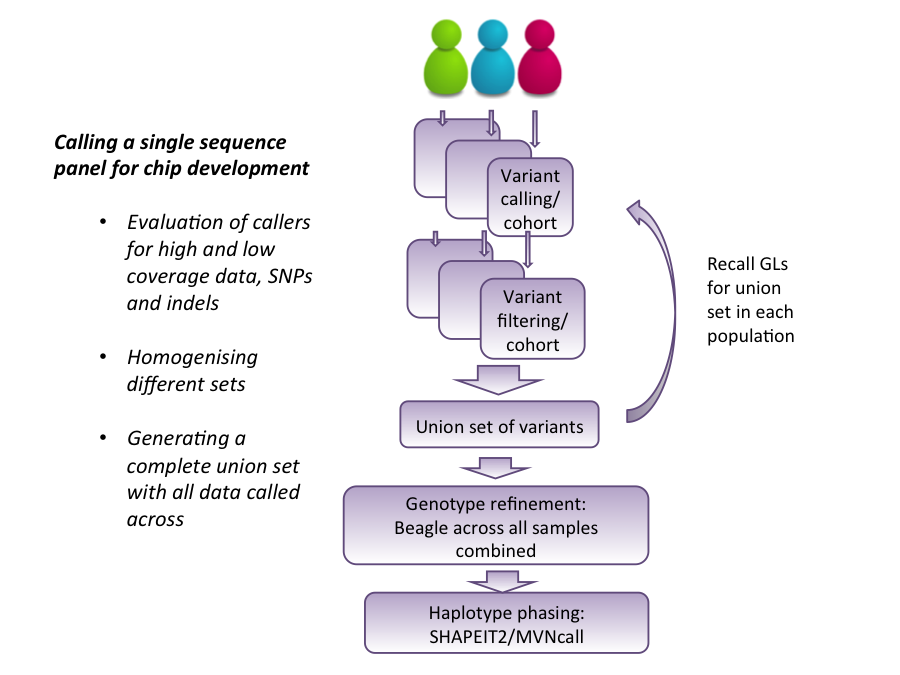
\includegraphics[width=0.8\textwidth]{calling}
\end{figure}
